% !TeX root = ../main.tex
% Add the above to each chapter to make compiling the PDF easier in some editors.

\chapter{Skin- and Blood-Light Interaction}\label{chapter:Skin- and Blood-Light Interaction}


\section{Skin-Light Interaction}

The relationship between an optical radiation and human skin depends
on the absorption and scattering properties of three skin layers, listing from the outside: epidermis, dermis, and hypodermis \parencite{skin}.
 
The structures and component chromophores of these layers determine the behaviour of radiation. Understanding the penetration of optical radiation can be achieved by studying and analysing the wavelength-dependent interactions of light with skin. For example, melanin exhibits maximum absorption in the UV and blue spectral
ranges, whereas blood absorbs blue and yellow light. The chromophores, such as melanin, blood, water, and lipid determine skin absorption \parencite{skin1}.
We will focus on the epidermis and dermis as the blood vessels are contained in the dermis

\subsubsection{Absorption and Scattering Properties of Epidermis and Dermis in The NIR Spectrum}

As the outermost skin layer, the epidermis forms the actual protective covering against environmental influences. The average thickness of epidermis is approximately 0.1 mm. However, on the face it maybe as thin as 0.02 mm, while on the soles of the feet it is as thick as 1–5 mm. Absorption and scattering of epidermis in the visible and NIR spectral ranges are defined almost exclusively by its melanin, the protein that adds pigment to skin, and water contents, respectively \parencite{skin1}.

The next layer is dermis, it is composed of gel-like and elastic materials, water, and, primarily, collagen. Embedded in this layer are systems and structures like lymph channels, blood vessels, nerve fibres, and muscle cells. Blood and water content define the absorptive properties of dermis in the visible and NIR range\parencite{skin1}.

Absorption and scattering coefficients of skin layers are shown in \autoref{fig:epidermis} and \autoref{fig:dermis} below \parencite{skin1}. The graphs demonstrate that the scattering and absorption of the first two skin layers decrease with the increasing wavelength. Which means light transmission increases with increasing wavelength.


\begin{figure}[H]
\centering
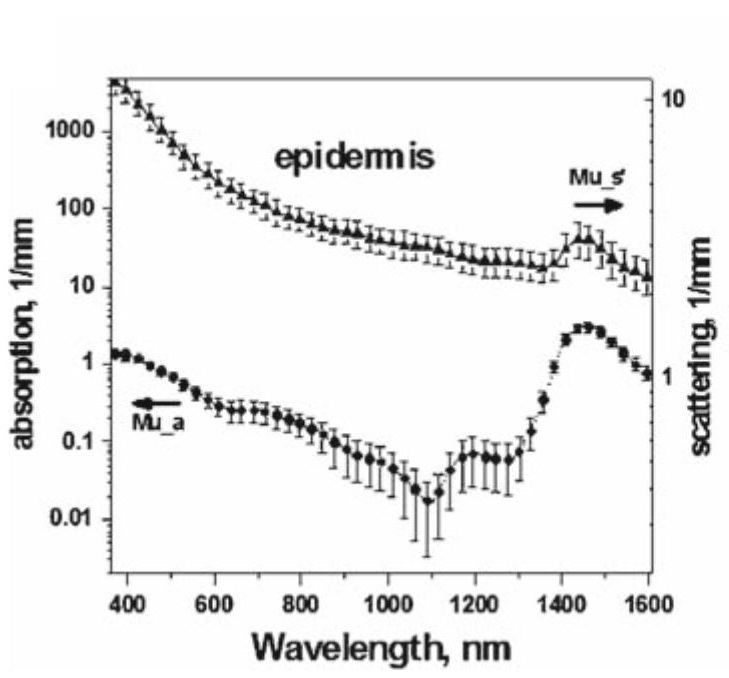
\includegraphics[scale=0.5]{figures/epidermis.JPG}
\captionsetup{justification=centering}
\caption[Optical properties of epidermis]{Optical properties of epidermis, Triangles – reduced scattering coefficients, circles absorption coefficients, bars – standard errors. Averaged over 7 samples.}\label{fig:epidermis}
\end{figure}





\begin{figure}[H]
\centering
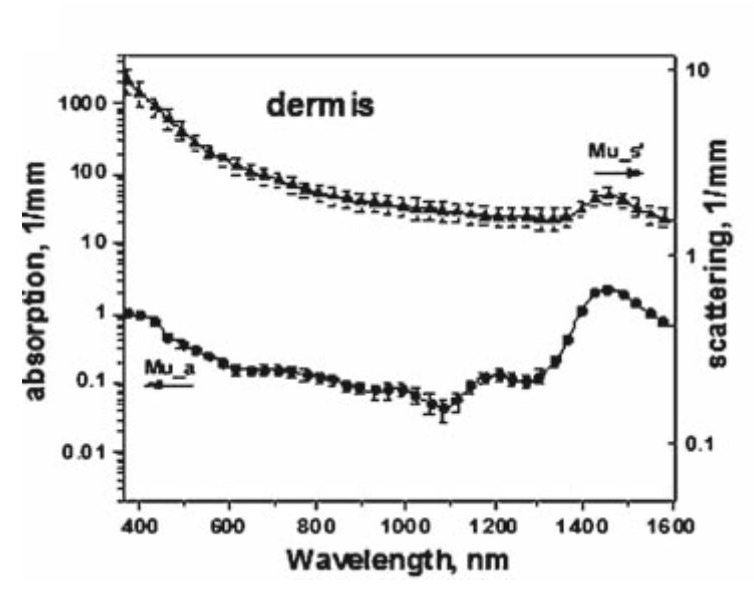
\includegraphics[scale=0.5]{figures/dermis.JPG}
\captionsetup{justification=centering}
\caption[Optical properties of dermis]{Optical properties of dermis. Triangles – reduced scattering coefficients,  circles absorption coefficients, bars – standard errors. Averaged over 8 samples.}\label{fig:dermis}
\end{figure}


\section{Blood-Light Interaction}


The optical properties of human blood under normal physiological conditions are largely determined by light interactions with plasma and red blood cells \parencite{opticsOfBlood}, which account for 99\% of the cellular elements \parencite{opticsOfBlood1}. 
The effects of the optical properties of WBCs and platelets on the light scattering and absorption by whole blood are considered negligible \parencite{opticsOfBlood}.

\subsubsection{Absorption and Scattering Properties of Red Blood Cells in the NIR Spectrum}
Red blood cells have a thin plasma membrane that encloses mainly a haemoglobin solution. The absorption and scattering of light by the RBCs are two to three orders of magnitude higher than those of the other blood components \parencite{opticsOfBlood1}. The light scattered by a single RBC depends on
its shape, volume, refractive index and orientation \parencite{opticsOfBlood1}. However, the absorption of light by the RBCs is dominated by haemoglobin in its functional, oxygen-binding, forms, namely oxyhaemoglobin and deoxyhaemoglobin.
The  \autoref{fig:blood} below shows a remarkable difference in absorption rates between oxygenated and deoxygenated blood within the wavelength range from 800 to 1150 nm.


\begin{figure}[H]
\centering
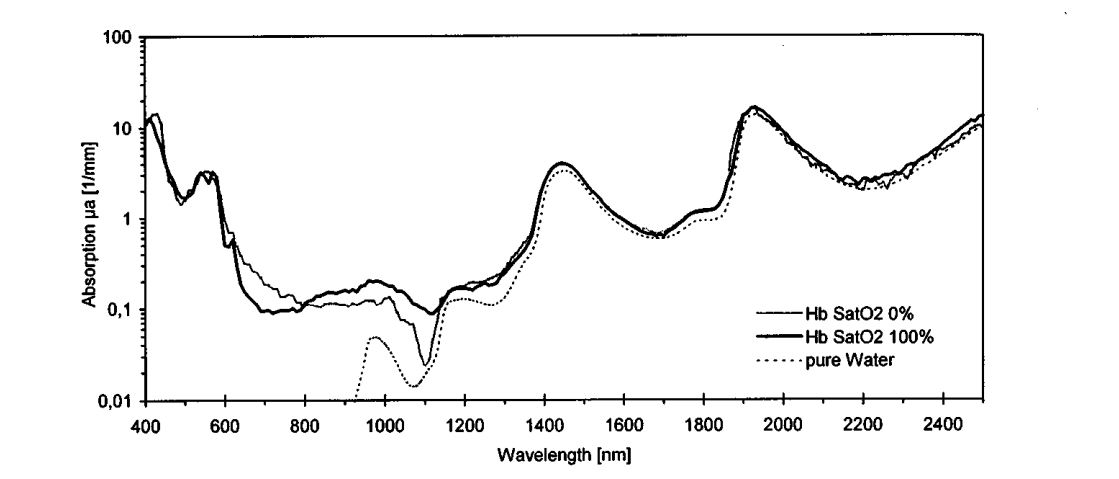
\includegraphics[scale=0.5]{figures/blood.JPG}
\caption[The absorption spectrum of oxygenated and deoxygenated diluted blood]{The absorption spectrum of oxygenated and deoxygenated diluted blood.}\label{fig:blood}
\end{figure}

\section{Conclusion: Wavelength Selection}
The goal of studying skin- and blood-light interaction is to analyse the absorption and scattering properties in both skin and light and eventually select the optimal wavelength to be used in the hardware extension. In summary, the optimal wavelength is the one that maximizes the skin, specifically the first layer, the epidermis, penetration, as well as the absorption of oxygenated blood, specifically oxyhaemoglobin. Due to the fact the veins carry only oxygenated blood, the selected wavelength should also maximize the difference in absorption rates between oxygenated and deoxygenated blood, which can enhance the contrast and the overall result. It is necessary to take into account the optical path of light traveling from the light source through the first skin layer, the epidermis, and then through the dermis which contains the vessels.  The light is then absorbed by the haemoglobin in RBCs in the oxygenated blood carried through the veins, but reflected/ scattered by the surrounding tissues.

The maximum value of epidermis light penetration is equivalent to the minimum value of light absorption. The graph \autoref{fig:epidermis} shows that the absorption of epidermis decreases with increasing wavelength and has minima at wavelength 1100nm.

The \autoref{fig:blood} demonstrates a maximum absorption value of blood at wavelengths 1500 and 2000 nm but as shown in \autoref{fig:epidermis} the light will not reach the blood or even the dermis at all as of the increased absorption of the epidermis at these wavelengths. Additionally, there is no difference in absorption between oxygenated and deoxygenated blood at these wavelengths.

Following from the discussion above, the wavelength in which the light can penetrate the epidermis but gets absorbed by oxyhaemoglobin lies in the range from 800 to 1100 nm, optimally at 1100nm.